% Created by tikzDevice version 0.7.0 on 2014-04-27 13:00:13
% !TEX encoding = UTF-8 Unicode
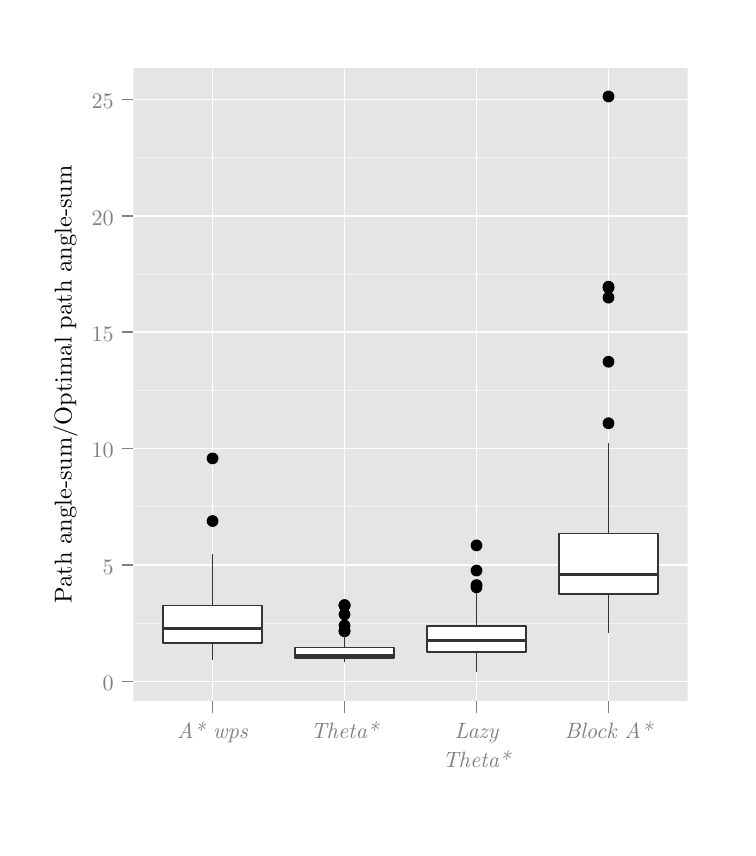
\begin{tikzpicture}[x=1pt,y=1pt]
\definecolor[named]{fillColor}{rgb}{1.00,1.00,1.00}
\path[use as bounding box,fill=fillColor,fill opacity=0.00] (0,0) rectangle (252.94,289.08);
\begin{scope}
\path[clip] (  0.00,  0.00) rectangle (252.94,289.08);
\definecolor[named]{drawColor}{rgb}{1.00,1.00,1.00}
\definecolor[named]{fillColor}{rgb}{1.00,1.00,1.00}

\path[draw=drawColor,line width= 0.6pt,line join=round,line cap=round,fill=fillColor] (  0.00, -0.00) rectangle (252.94,289.08);
\end{scope}
\begin{scope}
\path[clip] ( 38.20, 45.78) rectangle (238.49,274.63);
\definecolor[named]{fillColor}{rgb}{0.90,0.90,0.90}

\path[fill=fillColor] ( 38.20, 45.78) rectangle (238.49,274.63);
\definecolor[named]{drawColor}{rgb}{0.95,0.95,0.95}

\path[draw=drawColor,line width= 0.3pt,line join=round] ( 38.20, 73.89) --
	(238.49, 73.89);

\path[draw=drawColor,line width= 0.3pt,line join=round] ( 38.20,115.95) --
	(238.49,115.95);

\path[draw=drawColor,line width= 0.3pt,line join=round] ( 38.20,158.00) --
	(238.49,158.00);

\path[draw=drawColor,line width= 0.3pt,line join=round] ( 38.20,200.05) --
	(238.49,200.05);

\path[draw=drawColor,line width= 0.3pt,line join=round] ( 38.20,242.11) --
	(238.49,242.11);
\definecolor[named]{drawColor}{rgb}{1.00,1.00,1.00}

\path[draw=drawColor,line width= 0.6pt,line join=round] ( 38.20, 52.87) --
	(238.49, 52.87);

\path[draw=drawColor,line width= 0.6pt,line join=round] ( 38.20, 94.92) --
	(238.49, 94.92);

\path[draw=drawColor,line width= 0.6pt,line join=round] ( 38.20,136.97) --
	(238.49,136.97);

\path[draw=drawColor,line width= 0.6pt,line join=round] ( 38.20,179.03) --
	(238.49,179.03);

\path[draw=drawColor,line width= 0.6pt,line join=round] ( 38.20,221.08) --
	(238.49,221.08);

\path[draw=drawColor,line width= 0.6pt,line join=round] ( 38.20,263.13) --
	(238.49,263.13);

\path[draw=drawColor,line width= 0.6pt,line join=round] ( 66.81, 45.78) --
	( 66.81,274.63);

\path[draw=drawColor,line width= 0.6pt,line join=round] (114.50, 45.78) --
	(114.50,274.63);

\path[draw=drawColor,line width= 0.6pt,line join=round] (162.19, 45.78) --
	(162.19,274.63);

\path[draw=drawColor,line width= 0.6pt,line join=round] (209.88, 45.78) --
	(209.88,274.63);
\definecolor[named]{fillColor}{rgb}{0.00,0.00,0.00}

\path[fill=fillColor] ( 66.81,110.80) circle (  2.13);

\path[fill=fillColor] ( 66.81,133.43) circle (  2.13);
\definecolor[named]{drawColor}{rgb}{0.20,0.20,0.20}
\definecolor[named]{fillColor}{rgb}{0.20,0.20,0.20}

\path[draw=drawColor,line width= 0.6pt,line join=round,fill=fillColor] ( 66.81, 80.28) -- ( 66.81, 98.82);

\path[draw=drawColor,line width= 0.6pt,line join=round,fill=fillColor] ( 66.81, 66.79) -- ( 66.81, 60.41);
\definecolor[named]{fillColor}{rgb}{1.00,1.00,1.00}

\path[draw=drawColor,line width= 0.6pt,line join=round,line cap=round,fill=fillColor] ( 48.93, 80.28) --
	( 48.93, 66.79) --
	( 84.69, 66.79) --
	( 84.69, 80.28) --
	( 48.93, 80.28) --
	cycle;
\definecolor[named]{fillColor}{rgb}{0.20,0.20,0.20}

\path[draw=drawColor,line width= 1.1pt,line join=round,fill=fillColor] ( 48.93, 71.95) -- ( 84.69, 71.95);
\definecolor[named]{fillColor}{rgb}{0.00,0.00,0.00}

\path[fill=fillColor] (114.50, 70.96) circle (  2.13);

\path[fill=fillColor] (114.50, 80.40) circle (  2.13);

\path[fill=fillColor] (114.50, 77.05) circle (  2.13);

\path[fill=fillColor] (114.50, 71.12) circle (  2.13);

\path[fill=fillColor] (114.50, 80.30) circle (  2.13);

\path[fill=fillColor] (114.50, 73.07) circle (  2.13);

\path[fill=fillColor] (114.50, 80.37) circle (  2.13);
\definecolor[named]{fillColor}{rgb}{0.20,0.20,0.20}

\path[draw=drawColor,line width= 0.6pt,line join=round,fill=fillColor] (114.50, 65.15) -- (114.50, 70.06);

\path[draw=drawColor,line width= 0.6pt,line join=round,fill=fillColor] (114.50, 61.39) -- (114.50, 59.73);
\definecolor[named]{fillColor}{rgb}{1.00,1.00,1.00}

\path[draw=drawColor,line width= 0.6pt,line join=round,line cap=round,fill=fillColor] ( 96.62, 65.15) --
	( 96.62, 61.39) --
	(132.38, 61.39) --
	(132.38, 65.15) --
	( 96.62, 65.15) --
	cycle;
\definecolor[named]{fillColor}{rgb}{0.20,0.20,0.20}

\path[draw=drawColor,line width= 1.1pt,line join=round,fill=fillColor] ( 96.62, 62.34) -- (132.38, 62.34);
\definecolor[named]{fillColor}{rgb}{0.00,0.00,0.00}

\path[fill=fillColor] (162.19,102.01) circle (  2.13);

\path[fill=fillColor] (162.19, 87.67) circle (  2.13);

\path[fill=fillColor] (162.19, 86.84) circle (  2.13);

\path[fill=fillColor] (162.19, 92.91) circle (  2.13);
\definecolor[named]{fillColor}{rgb}{0.20,0.20,0.20}

\path[draw=drawColor,line width= 0.6pt,line join=round,fill=fillColor] (162.19, 72.87) -- (162.19, 84.74);

\path[draw=drawColor,line width= 0.6pt,line join=round,fill=fillColor] (162.19, 63.57) -- (162.19, 56.18);
\definecolor[named]{fillColor}{rgb}{1.00,1.00,1.00}

\path[draw=drawColor,line width= 0.6pt,line join=round,line cap=round,fill=fillColor] (144.30, 72.87) --
	(144.30, 63.57) --
	(180.07, 63.57) --
	(180.07, 72.87) --
	(144.30, 72.87) --
	cycle;
\definecolor[named]{fillColor}{rgb}{0.20,0.20,0.20}

\path[draw=drawColor,line width= 1.1pt,line join=round,fill=fillColor] (144.30, 67.55) -- (180.07, 67.55);
\definecolor[named]{fillColor}{rgb}{0.00,0.00,0.00}

\path[fill=fillColor] (209.88,146.14) circle (  2.13);

\path[fill=fillColor] (209.88,264.22) circle (  2.13);

\path[fill=fillColor] (209.88,168.36) circle (  2.13);

\path[fill=fillColor] (209.88,195.08) circle (  2.13);

\path[fill=fillColor] (209.88,191.52) circle (  2.13);

\path[fill=fillColor] (209.88,195.47) circle (  2.13);
\definecolor[named]{fillColor}{rgb}{0.20,0.20,0.20}

\path[draw=drawColor,line width= 0.6pt,line join=round,fill=fillColor] (209.88,106.28) -- (209.88,139.04);

\path[draw=drawColor,line width= 0.6pt,line join=round,fill=fillColor] (209.88, 84.39) -- (209.88, 70.51);
\definecolor[named]{fillColor}{rgb}{1.00,1.00,1.00}

\path[draw=drawColor,line width= 0.6pt,line join=round,line cap=round,fill=fillColor] (191.99,106.28) --
	(191.99, 84.39) --
	(227.76, 84.39) --
	(227.76,106.28) --
	(191.99,106.28) --
	cycle;
\definecolor[named]{fillColor}{rgb}{0.20,0.20,0.20}

\path[draw=drawColor,line width= 1.1pt,line join=round,fill=fillColor] (191.99, 91.41) -- (227.76, 91.41);
\end{scope}
\begin{scope}
\path[clip] (  0.00,  0.00) rectangle (252.94,289.08);
\definecolor[named]{drawColor}{rgb}{0.50,0.50,0.50}

\node[text=drawColor,anchor=base east,inner sep=0pt, outer sep=0pt, scale=  0.80] at ( 31.08, 49.56) {0};

\node[text=drawColor,anchor=base east,inner sep=0pt, outer sep=0pt, scale=  0.80] at ( 31.08, 91.61) {5};

\node[text=drawColor,anchor=base east,inner sep=0pt, outer sep=0pt, scale=  0.80] at ( 31.08,133.67) {10};

\node[text=drawColor,anchor=base east,inner sep=0pt, outer sep=0pt, scale=  0.80] at ( 31.08,175.72) {15};

\node[text=drawColor,anchor=base east,inner sep=0pt, outer sep=0pt, scale=  0.80] at ( 31.08,217.77) {20};

\node[text=drawColor,anchor=base east,inner sep=0pt, outer sep=0pt, scale=  0.80] at ( 31.08,259.83) {25};
\end{scope}
\begin{scope}
\path[clip] (  0.00,  0.00) rectangle (252.94,289.08);
\definecolor[named]{drawColor}{rgb}{0.50,0.50,0.50}

\path[draw=drawColor,line width= 0.6pt,line join=round] ( 33.93, 52.87) --
	( 38.20, 52.87);

\path[draw=drawColor,line width= 0.6pt,line join=round] ( 33.93, 94.92) --
	( 38.20, 94.92);

\path[draw=drawColor,line width= 0.6pt,line join=round] ( 33.93,136.97) --
	( 38.20,136.97);

\path[draw=drawColor,line width= 0.6pt,line join=round] ( 33.93,179.03) --
	( 38.20,179.03);

\path[draw=drawColor,line width= 0.6pt,line join=round] ( 33.93,221.08) --
	( 38.20,221.08);

\path[draw=drawColor,line width= 0.6pt,line join=round] ( 33.93,263.13) --
	( 38.20,263.13);
\end{scope}
\begin{scope}
\path[clip] (  0.00,  0.00) rectangle (252.94,289.08);
\definecolor[named]{drawColor}{rgb}{0.50,0.50,0.50}

\path[draw=drawColor,line width= 0.6pt,line join=round] ( 66.81, 41.51) --
	( 66.81, 45.78);

\path[draw=drawColor,line width= 0.6pt,line join=round] (114.50, 41.51) --
	(114.50, 45.78);

\path[draw=drawColor,line width= 0.6pt,line join=round] (162.19, 41.51) --
	(162.19, 45.78);

\path[draw=drawColor,line width= 0.6pt,line join=round] (209.88, 41.51) --
	(209.88, 45.78);
\end{scope}
\begin{scope}
\path[clip] (  0.00,  0.00) rectangle (252.94,289.08);
\definecolor[named]{drawColor}{rgb}{0.50,0.50,0.50}

\node[text=drawColor,anchor=base,inner sep=0pt, outer sep=0pt, scale=  0.80] at ( 66.81, 32.05) {{\em A* wps}};

\node[text=drawColor,anchor=base,inner sep=0pt, outer sep=0pt, scale=  0.80] at (114.50, 32.05) {{\em Theta*}};

\node[text=drawColor,anchor=base,inner sep=0pt, outer sep=0pt, scale=  0.80] at (162.19, 32.05) {{\em Lazy}};

\node[text=drawColor,anchor=base,inner sep=0pt, outer sep=0pt, scale=  0.80] at (162.19, 21.69) {{\em Theta*}};

\node[text=drawColor,anchor=base,inner sep=0pt, outer sep=0pt, scale=  0.80] at (209.88, 32.05) {{\em Block A*}};
\end{scope}
\begin{scope}
\path[clip] (  0.00,  0.00) rectangle (252.94,289.08);
\definecolor[named]{drawColor}{rgb}{0.00,0.00,0.00}

\node[text=drawColor,rotate= 90.00,anchor=base,inner sep=0pt, outer sep=0pt, scale=  0.88] at ( 15.90,160.20) {Path angle-sum/Optimal path angle-sum};
\end{scope}
\end{tikzpicture}
